% ===========================================================================
% CAPÍTULO 3: DESARROLLO
% ===========================================================================

\section{Preparación del entorno de desarrollo}

Durante este trabajo se utilizó una máquina virtual con un sistema operativo Linux
(Ubuntu/Debian) como entorno de desarrollo principal. Esta elección respondió a dos
motivos prácticos. La máquina virtual puede dejarse trabajando de forma indefinida, lo
que resulta necesario para las compilaciones prolongadas de la herramienta de síntesis.
Además, se le pueden asignar muchos más recursos de memoria y almacenamiento de los que
estarían disponibles en un equipo de trabajo convencional.

Se siguieron los siguientes pasos para dejar operativo el
entorno de desarrollo.

\subsection{Instalación de Vivado y Vitis}

Para el desarrollo de la lógica programable (PL) y la generación de imágenes de arranque, se
utilizaron las herramientas oficiales de AMD: Vivado Design Suite y Vitis Unified
Software Platform. Vivado se empleó para el diseño a nivel de hardware y la generación del
\textit{bitstream}, mientras que Vitis se utilizó para empaquetar los binarios y generar la imagen de
arranque (BOOT.BIN). Ambas estaban instaladas previamente en la máquina virtual, en su
\textbf{versión 2025.1}, que es la que se mantuvo durante todo el trabajo y con la que son
coherentes los componentes de arranque precompilados empleados más adelante.

\subsection{Instalación de RTEMS}

RTEMS (versión 7) se compiló desde código fuente en lugar de partir de binarios precompilados,
siguiendo la guía \textit{Quick Start} del manual de usuario oficial del
proyecto~\cite{rtems_quickstart} y empleando la herramienta RTEMS Source Builder
(RSB)~\cite{rtems_rsb}. Un binario genérico no habría garantizado la combinación exacta que este
trabajo necesitaba: un \textit{toolchain} cruzado para la arquitectura AArch64, el BSP
\texttt{zynqmp\_apu} concreto de la ZCU102 y el soporte de multiprocesamiento simétrico (SMP)
habilitado explícitamente en la configuración del núcleo. Sobre ese control se apoyó después la
integración del driver propio del transceptor.

El entorno recién compilado se validó sobre el emulador QEMU (\texttt{qemu-system-aarch64}) con la
máquina \texttt{xlnx-zcu102}, ejecutando los ejemplos \texttt{hello.exe} y
\texttt{dhrystone.exe}~\cite{weicker1984dhrystone} que el propio BSP incluye: confirman que el
arranque y la consola serie funcionan y que el \textit{toolchain} genera código funcional.

\subsection{Validación del flujo de desarrollo de extremo a extremo} \label{sec:flujo_extremo_a_extremo}

Con las herramientas ya instaladas, quedaba por comprobar que encajaban entre sí. Antes de
abordar el transceptor serie se recorrió el flujo completo con el ejemplo más pequeño posible:
una \textbf{puerta AND}. La puerta se describió en VHDL y se sintetizó en la \textbf{PL}, y en el
\textbf{PS} se escribió un programa de RTEMS que excitaba todas las combinaciones de sus entradas,
leía la salida por AXI e imprimía cada resultado por la consola serie. La dificultad no está en la
puerta, sino en el camino que lleva un \textit{bitstream} y un programa en C hasta la ZCU102.

Ese camino se reduce a dejar dos ficheros en la tarjeta SD desde la que arranca la placa. Uno es
la \textbf{imagen de arranque}, que reúne el \textit{bitstream} de la PL y todo el software que
levanta el sistema antes de que exista aplicación alguna; el otro es la \textbf{imagen de la
aplicación} que después ejecuta el PS. La primera se construye con Vivado y Vitis, la segunda
compilando la aplicación de RTEMS. El procedimiento paso a paso --- la descripción VHDL, el
\textit{Block Design}, los componentes de la imagen de arranque, la posición del conmutador de la
placa y el volcado del barrido --- se recoge en el apartado~\ref{anxC:flujo_and} del Anexo~\ref{anx:rtl}, y el
código de ambas mitades, la descripción VHDL y la aplicación de RTEMS, está en
\texttt{tfm/00\_docs/AND\_example} dentro del
repositorio~\cite{repo_tfm}.

El barrido de la tabla de verdad salió por la consola serie con la salida a uno únicamente cuando
ambas entradas valían uno. Fue la primera confirmación de que la cadena entera funcionaba: el VHDL
sintetizado en la PL, la imagen de arranque, la aplicación de RTEMS y la comunicación
PS$\leftrightarrow$PL por AXI. De esa puesta en marcha salió además un detalle que reaparece más
adelante: RTEMS desconoce a priori las direcciones de la PL, así que hay que declarar el rango
\texttt{0xA0000000}--\texttt{0xA01FFFFF} como memoria de periférico nada más arrancar la tarea
\texttt{Init}. Sin ese mapeado, el primer acceso a los GPIO aborta la ejecución. El mismo problema
vuelve en el apartado~\ref{sec:testing_driver} del capítulo~\ref{cap:hardware}, ya resuelto como
\texttt{mmu\_map\_pl\_axi\_early()}.

\textbf{Automatización del flujo.} Lo que hizo falta corregir no fue el ejemplo, sino el coste de
repetirlo. Cada iteración obliga a sintetizar el diseño en Vivado, crear y compilar una plataforma
y una aplicación nuevas en Vitis, ensamblar la imagen de arranque, compilar la imagen de RTEMS,
copiar los ficheros a la tarjeta y arrancar la placa: \textbf{casi una hora de media}. Y cuando la
placa no arranca, no da ninguna indicación del motivo. Agrava el problema que Vitis reutiliza
artefactos ya compilados: un diseño nuevo no siempre llega a la imagen final, la placa se comporta
como antes del cambio en el VHDL y limpiar y recompilar no da un resultado fiable. De ahí la regla
que se adoptó para el resto del trabajo, plataforma y aplicación nuevas ante cualquier cambio en
la PL, que es más lenta pero garantiza que la imagen corresponde al hardware recién sintetizado.

Con ese tiempo por iteración, automatizar dejó de ser una comodidad. Se escribieron tres
herramientas que, entre las tres, cubren el camino entero y están disponibles en el
repositorio~\cite{repo_tfm}:

\begin{itemize}
    \item \texttt{make\_img.sh} compila la aplicación de RTEMS y la deja empaquetada en el formato
    de imagen que el gestor de arranque espera encontrar en la tarjeta.

    \item \texttt{automate\_ymodem\_update.py} ahorra el vaivén de la tarjeta SD. En lugar de
    sacarla de la placa, copiar el fichero desde el ordenador y volver a montarla, el script manda
    la imagen a la placa por el mismo cable USB que hace de consola y la deja escrita en la
    tarjeta. Probar un cambio en la aplicación se quedó en lanzar el script y pulsar el botón que
    reinicia el procesador sin cortar la alimentación.

    \item \texttt{generate\_boot.sh} cubre la mitad que faltaba, la de la imagen de arranque.
    Encadena de forma desatendida los pasos que antes se hacían navegando por los asistentes
    gráficos de Vivado y Vitis, donde olvidar un componente o arrastrar un artefacto antiguo basta
    para que la placa no arranque sin decir por qué. Admite empezar desde el proyecto de Vivado o
    desde un diseño ya sintetizado, según lo que haya cambiado.
\end{itemize}

El tiempo de iteración pasó así de una sesión larga de interacción gráfica a un par de órdenes en
el terminal, con la garantía de que lo que arranca en la placa corresponde al hardware recién
sintetizado. Este flujo quedó establecido como procedimiento estándar para el resto del trabajo.

% ---------------------------------------------------------------------------
\section{Diseño del transceptor serie configurable (PL)} \label{sec:transceptor_pl}
% ---------------------------------------------------------------------------

El transceptor serie se diseñó para ser altamente configurable y adaptable a cualquier
dispositivo, debido a que se desconocían los dispositivos finales que iban a estar conectados
al OBC.

El transceptor completo consta de varios bloques conectados entre sí. Los bloques
fundamentales son:

\begin{itemize}
    \item \textbf{Oscilador controlado numéricamente} (\texttt{NCO.vhd}): proporciona la señal
    de temporización de bit para las 54 velocidades de bus soportadas. El transmisor y el
    receptor instancian uno cada uno para poder trabajar a cualquiera de ellas.
    \item \textbf{Transmisor} (\texttt{TX\_CONFIGURABLE\_SERIAL.vhd}): serializa y emite las
    tramas, y gobierna la señal de \textit{Driver Enable} del transceptor físico.
    \item \textbf{Receptor} (\texttt{RX\_CONFIGURABLE\_SERIAL.vhd}): detecta el inicio de trama,
    muestrea la línea, comprueba paridad y bit de parada y valida la palabra recibida.
    \item \textbf{Registro de desplazamiento} (\texttt{ShiftRegister.vhd}): convierte a paralelo
    los bits recibidos. Incorpora la lógica necesaria para adaptarse a todas las combinaciones
    de número y orden de los bits.
    \item \textbf{Memoria FIFO}: almacena las palabras recibidas hasta que el PS las lee.
    \item \textbf{Bloque de canal} (\texttt{CONFIGURABLE\_SERIAL.vhd}): integra los bloques
    anteriores y añade la lógica de acoplamiento entre ellos.
    \item \textbf{Bloque \textit{top}} (\texttt{CONFIGURABLE\_SERIAL\_TOP.vhd}): empaqueta el
    canal completo en los dos vectores que lo conectan al PS.
\end{itemize}

Los parámetros configurables son:

\begin{itemize}
    \item Velocidad de bus, o \textit{baudrate}, desde 50 hasta 4\,000\,000~baudios.
    \item Número de bits de parada, o \textit{stop bits}, que marcan el final de la trama y
    devuelven la línea a reposo: 1, 1,5 o 2.
    \item Modo de paridad: par, impar, marca, espacio o deshabilitada. La paridad es un único bit
    de comprobación que iguala a par o a impar el número de unos de la palabra.
    \item Orden de los bits, empezando por el menos significativo (LSB) o por el más
    significativo (MSB).
    \item Número de bits de datos, entre 5 y 9.
\end{itemize}

Los siguientes apartados describen esos bloques uno a uno, siguiendo el camino que recorre un
dato. Primero, el NCO, que marca la base de tiempos: el transmisor y el receptor tienen cada
uno el suyo. Después, el transmisor y el receptor. Y por último, los bloques que los conectan
al PS. El
apartado~\ref{sec:bloque_canal} cierra con el diagrama de conjunto
(figura~\ref{fig:transceptor_bloques}), cuando ya se han presentado todas sus piezas.

\subsection{Oscilador controlado numéricamente (NCO)}

El transmisor y el receptor tienen cada uno su propia base de tiempos, un NCO que se describe
en primer lugar porque su salida, el \textit{tick}, es la referencia con la que cada uno mide el
tiempo de bit.

El transceptor debía poder variar su velocidad en tiempo de ejecución sobre un rango muy amplio
de baudrates, y un divisor entero del reloj de la FPGA no puede generar con exactitud la mayoría
de esas frecuencias. La solución fue un \textbf{oscilador controlado numéricamente} (NCO), un tipo
de circuito que corrige periódicamente el desfase acumulado por esa imprecisión, y que se diseñó
a medida para las necesidades del proyecto: genera la señal de \textit{enable} al baudrate
seleccionado de entre 54 valores de velocidad almacenados en una tabla de verdad.

El bloque expone una interfaz mínima: además del reloj, una entrada de reset asíncrono activo a
nivel bajo (\texttt{rst}), una habilitación (\texttt{en}), el selector de velocidad
(\texttt{baud\_sel}, 6 bits), un selector de modo (\texttt{half\_mode}) y la salida de
temporización (\texttt{tick}). El número de bits del acumulador es un parámetro \textit{generic},
fijado a 32.

El circuito consiste en un sumador acumulador: para cada frecuencia seleccionada, se tiene
calculado un incremento concreto que depende del número de bits del sumador. Cuantos más
bits tenga este sumador, mejor precisión se consigue. En esta implementación se han
utilizado 32 bits. El incremento se suma y acumula en cada período de reloj. Cuando el
sumador se desborda, se utiliza el bit de \textit{carry\_out} como \textit{tick} del NCO. Este \textit{tick} se genera
a la frecuencia deseada, y el mecanismo de acumulación garantiza que el error promedio sea
inferior al de un divisor entero simple.

Los incrementos no se almacenan como literales: los calcula en tiempo de síntesis una función
que evalúa $\mathrm{inc} = \lfloor 2^{32} \cdot f_{\mathrm{baud}} / f_{\mathrm{clk}} \rfloor$ para
cada entrada de la tabla, de modo que basta cambiar la constante de frecuencia de reloj para
reajustar las 54 velocidades. La tabla tiene dos columnas por entrada: el incremento nominal y el
de doble frecuencia, que selecciona \texttt{half\_mode}. Este segundo valor es el que permite medir
semiperíodos de bit, algo que necesitan tanto el transmisor, en el campo de parada, como el
receptor, en el bit de inicio. Tabularlo en lugar de duplicar el primero evita arrastrar
multiplicado por dos el error de truncamiento del incremento nominal.

Las dos entradas de control restantes son las que permiten a la máquina de estados del
transmisor y a la del receptor anclar la fase de su temporizador: \texttt{rst} pone a cero acumulador y
salida, con lo que el \textit{tick} arranca alineado con el inicio de la trama, y \texttt{en}
congela el acumulador en los estados en los que no se necesita temporización, evitando que la fase
derive entre tramas. La salida \texttt{tick} está registrada, por lo que aparece un ciclo de reloj
después del desbordamiento.

Para validar su funcionamiento se desarrolló un \textit{testbench} dedicado,
\texttt{tb\_NCO.vhd} (en \texttt{tfm/01\_ip\_serie/testbench/} del repositorio del
proyecto~\cite{repo_tfm}), que barre las \textbf{29 velocidades del rango de uso} (de 9\,600 a
3,6864~Mbaudios) en sus \textbf{dos modos} de temporización, y mide en cada punto la frecuencia
real del \textit{tick} promediando 200 períodos tras descartar los diez primeros. Son 58 medidas
independientes. Las entradas de la tabla por debajo de 9\,600~baudios y la de 4~Mbaudios no se
ejercitan, por quedar la primera fuera del uso previsto y exigir la segunda un tiempo de simulación
desproporcionado. La transcripción siguiente recoge el principio y el final de la campaña:

\begin{lstlisting}[style=terminal, caption={Salida de la simulación de \texttt{tb\_NCO.vhd} (extracto)}]
---- Configuracion: 9600 half=0 baud=9600 ----
CFG=9600 expected=9600.0 Hz  measured=9600.002000 Hz  err=0.002000 Hz (0.2 ppm)
---- Configuracion: 9600 half=1 baud=9600 ----
CFG=9600 expected=19200.0 Hz  measured=19200.004000 Hz  err=0.004000 Hz (0.2 ppm)
---- Configuracion: 14400 half=0 baud=14400 ----
CFG=14400 expected=14400.0 Hz  measured=14399.988000 Hz  err=-0.012000 Hz (-0.8 ppm)
...
---- Configuracion: 115200 half=0 baud=115200 ----
CFG=115200 expected=115200.0 Hz  measured=115200.074000 Hz  err=0.074000 Hz (0.6 ppm)
---- Configuracion: 115200 half=1 baud=115200 ----
CFG=115200 expected=230400.0 Hz  measured=230400.148000 Hz  err=0.148000 Hz (0.6 ppm)
...
---- Configuracion: 3686400 half=0 baud=3686400 ----
CFG=3686400 expected=3686400.0 Hz  measured=3685956.506000 Hz  err=-443.494000 Hz (-120.3 ppm)
---- Configuracion: 3686400 half=1 baud=3686400 ----
CFG=3686400 expected=7372800.0 Hz  measured=7371913.012000 Hz  err=-886.988000 Hz (-120.3 ppm)
Fin del testbench: medidas completadas para todas las frecuencias.
\end{lstlisting}

De esa campaña procede la tabla~\ref{tab:nco} del Anexo~\ref{anx:rtl}, y su lectura valida el diseño: el peor
error de todo el rango es de 120~ppm (a 3,6864~Mbaudios), dos órdenes de magnitud por debajo de la
tolerancia habitual del $\pm$2\,\% de un receptor UART, y en la mayoría de las velocidades estándar
el error es nulo o inferior a 1~ppm. El NCO queda así acreditado como fuente de temporización
fiable para todo el rango de operación del transceptor.

\subsection{Transmisor}

El transmisor recibe una palabra en paralelo y la emite por la línea serie con el formato de
trama que fijan sus entradas de configuración. Sus puertos se recogen en la
tabla~\ref{tab:tx_puertos}.

\begin{table}[H]
    \centering
    \begin{tabular}{llp{0.55\textwidth}}
        \hline
        \textbf{Puerto} & \textbf{Dir.} & \textbf{Función} \\
        \hline
        \texttt{Clk}       & in  & Reloj del sistema, 100~MHz, activo por flanco de subida. \\
        \texttt{Reset}     & in  & Reset asíncrono del sistema, activo a nivel bajo. \\
        \texttt{Start}     & in  & Pulso de petición de transmisión. \\
        \texttt{Data}      & in  & Palabra a transmitir (9 bits, alineada en el LSB). \\
        \texttt{baud\_sel} & in  & Índice de velocidad dentro de la tabla del NCO (6 bits). \\
        \texttt{stop\_bit} & in  & Duración del campo de parada, en semiperíodos de bit
                                   (\texttt{010}~=~1, \texttt{011}~=~1,5, \texttt{100}~=~2). \\
        \texttt{parity}    & in  & Modo de paridad: par, impar, \textit{mark}, \textit{space}
                                   o deshabilitada. \\
        \texttt{bit\_order}& in  & Orden de emisión: \texttt{0}~=~LSB \textit{first},
                                   \texttt{1}~=~MSB \textit{first}. \\
        \texttt{data\_bits}& in  & Número de bits de datos (\texttt{000}--\texttt{100}
                                   $\rightarrow$ 5--9 bits). \\
        \texttt{EOT}       & out & Transmisor libre: a nivel alto únicamente en reposo. \\
        \texttt{DE}        & out & \textit{Driver Enable} del transceptor físico. \\
        \texttt{TX}        & out & Línea de transmisión serie. \\
        \hline
    \end{tabular}
    \caption{Puertos del transmisor \texttt{TX\_CONFIGURABLE\_SERIAL}.}
    \label{tab:tx_puertos}
\end{table}

Dispone además de un parámetro \textit{generic}, \texttt{DELAY\_CYCLES}, cuyo uso se detalla más
adelante.

\subsubsection{Máquina de estados}

La temporización del tiempo de bit y del semiperíodo de bit la proporciona el NCO, instanciado
dentro del propio transmisor: la FSM lo habilita, lo pone a cero y conmuta su entrada
\texttt{half\_mode} según el estado, y consume su salida \texttt{tick} como base de tiempos. El
comportamiento se organiza en siete estados:

\begin{itemize}
    \item \textbf{\texttt{Idle}}: estado de reposo. Mantiene la línea en alto, \texttt{EOT} a uno
    y el NCO detenido. Al llegar \texttt{Start} activa \texttt{DE}, pone a cero el contador de
    retardo y pasa a \texttt{PreDE}.

    \item \textbf{\texttt{PreDE}}: mantiene \texttt{DE} activo y la línea en reposo durante
    \texttt{DELAY\_CYCLES} ciclos de reloj, para dar tiempo al transceptor físico a habilitar su
    etapa de salida antes de que empiece la trama. Al cumplirse la cuenta se borra el contador de
    bits y se resetea el acumulador del NCO, con lo que la fase del temporizador arranca desde
    cero justo en el bit de inicio, sin arrastrar el desfase acumulado de la trama anterior. Hecho
    esto se pasa a \texttt{StartBit}.

    \item \textbf{\texttt{StartBit}}: fuerza la línea a nivel bajo durante un tiempo de bit
    completo. Con el primer \textit{tick} del NCO pasa a \texttt{SendData}.

    \item \textbf{\texttt{SendData}}: saca a la línea el bit seleccionado por el multiplexor de
    serialización y avanza el contador de bits con cada \textit{tick}. Cuando el contador alcanza
    el número de bits configurado, pasa a \texttt{ParityBit} presentando ya el bit de paridad o,
    si la paridad está deshabilitada (\texttt{parity}~=~\texttt{100}), directamente a
    \texttt{StopBit} con la línea en alto.

    \item \textbf{\texttt{ParityBit}}: mantiene el bit de paridad durante un tiempo de bit y pasa
    a \texttt{StopBit}.

    \item \textbf{\texttt{StopBit}}: mantiene la línea en alto y conmuta el NCO a
    \texttt{half\_mode}, que lo hace oscilar al doble de la velocidad seleccionada. Contando
    semiperíodos (dos, tres o cuatro según \texttt{stop\_bit}) se obtienen los tres campos de
    parada admitidos, incluido el de 1,5~bits, que no es expresable con una cuenta de bits enteros.
    Alcanzada la cuenta pasa a \texttt{PostDE}.

    \item \textbf{\texttt{PostDE}}: simétrico de \texttt{PreDE}. Mantiene \texttt{DE} activo y la
    línea en reposo otros tantos ciclos antes de volver a \texttt{Idle}, donde
    \texttt{DE} se libera.
\end{itemize}

\subsubsection{Lógica de apoyo a la máquina de estados}

La FSM se limita a secuenciar la trama y a generar señales de control. El trabajo de seleccionar
qué bit sale a la línea en cada momento recae en un camino de datos puramente combinacional que
la acompaña, y que evita tener que desplazar o rotar la palabra de entrada.

\textbf{Banco de contadores.} Tres contadores síncronos con habilitación y borrado independientes,
gobernados por la FSM: el de bits de datos (4 bits), el de semiperíodos del campo de parada
(3~bits) y el de retardo de \texttt{DE} (14~bits, suficiente para el valor por defecto de
\texttt{DELAY\_CYCLES}). Todos comparten el mismo proceso síncrono y el mismo reset asíncrono.

\textbf{Decodificador de anchura de palabra.} Traduce el código de \texttt{data\_bits}
(\texttt{000}--\texttt{100}) al número real de bits (5--9), que es el valor terminal con el que se
compara el contador de datos.

\textbf{Multiplexor de serialización.} Selecciona el bit a emitir a partir de la cuenta actual, en
tres etapas. La rama LSB \textit{first} es directa: el índice del contador es el índice del bit. La
rama MSB \textit{first} requiere cinco multiplexores distintos, uno por anchura de palabra, porque
el primer bit emitido depende del tamaño de la trama: es el bit~4 en una palabra de 5~bits y el
bit~8 en una de 9. Una segunda etapa elige entre esas cinco ramas según \texttt{data\_bits}, y una
tercera entre LSB y MSB \textit{first} según \texttt{bit\_order}. El resultado es que la palabra
permanece inmóvil en su registro de entrada durante toda la trama.

\textbf{Generador de paridad.} Una red de puertas XOR calcula la paridad de los bits activos, con
una expresión por cada anchura de palabra, y un multiplexor final aplica el modo configurado: paridad
par, su complemento para la impar, o las constantes uno y cero para los modos \textit{mark} y
\textit{space}.

\textbf{Reset del NCO.} La entrada de reset del NCO se combina con el reset global del sistema, de
modo que el temporizador se inicializa tanto cuando lo pide la FSM (antes de cada trama) como
cuando se resetea el transceptor completo.

\subsubsection{Retardo de establecimiento del \textit{Driver Enable}}

Los estados \texttt{PreDE} y \texttt{PostDE} se incorporaron después de la primera versión del
transmisor, al aparecer caracteres corruptos de forma ocasional en las primeras recepciones sobre
la placa CDHS. La hipótesis de partida era que \texttt{DE} conmutaba con demasiada rapidez en el
paso de transmisión a recepción y no dejaba establecerse al transceptor físico. Los dos estados
sitúan un margen configurable a ambos lados de la trama: \texttt{DE} se activa
\texttt{DELAY\_CYCLES} ciclos antes del bit de inicio y se libera otros tantos después del último
bit de parada. El valor por defecto es de 10\,000 ciclos, esto es, 100~$\mu$s con el reloj de
100~MHz. En simulación se reduce a una decena de ciclos mediante el \textit{generic} para no
alargar los \textit{testbench}, sin que ello afecte al valor de síntesis.

La medida no eliminó los caracteres corruptos, cuya causa estaba en el receptor y se aborda en el
apartado siguiente, pero los dos estados se conservaron: el margen es coherente con los tiempos
de habilitación que especifican los transceptores empleados y su coste, 200~$\mu$s por trama en el
peor caso, es despreciable frente al tiempo de trama salvo a las velocidades más altas.

\subsection{Receptor}

El receptor vigila la línea serie, recupera la temporización de bit a partir del flanco de inicio y
entrega los bits muestreados al registro de desplazamiento, señalando al final si la trama es
válida. Sus puertos se recogen en la tabla~\ref{tab:rx_puertos}. Las cinco entradas de
configuración son las mismas del transmisor y con idéntica codificación, por lo que ambos
comparten la palabra de configuración del canal.

\begin{table}[H]
    \centering
    \begin{tabular}{p{0.24\textwidth}lp{0.5\textwidth}}
        \hline
        \textbf{Puerto} & \textbf{Dir.} & \textbf{Función} \\
        \hline
        \texttt{Clk}, \texttt{Reset}    & in  & Reloj de 100~MHz y reset asíncrono activo a nivel
                                                bajo. \\
        \texttt{baud\_sel}, \texttt{stop\_bit}, \texttt{parity}, \texttt{bit\_order},
        \texttt{data\_bits}             & in  & Configuración del formato de trama, idéntica a la
                                                del transmisor. \\
        \texttt{LineRD\_in}             & in  & Línea de recepción, ya registrada por el bloque de
                                                canal. \\
        \texttt{shiftRegister\_Q}       & in  & Palabra normalizada que va acumulando el registro
                                                de desplazamiento, sobre la que se calcula la
                                                paridad esperada. \\
        \texttt{ERROR\_OK}              & in  & Borrado de las banderas de error. \\
        \texttt{PAR\_ERROR}             & out & Error de paridad. \\
        \texttt{FRAME\_ERROR}           & out & Error de trama (bit de parada ausente). \\
        \texttt{Valid\_out}             & out & Pulso de bit válido; habilita el registro de
                                                desplazamiento. \\
        \texttt{Code\_out}              & out & Valor muestreado de la línea, que entra al registro
                                                de desplazamiento. \\
        \texttt{Store\_out}             & out & Pulso de escritura de la palabra completa en la
                                                FIFO. \\
        \hline
    \end{tabular}
    \caption{Puertos del receptor \texttt{RX\_CONFIGURABLE\_SERIAL}.}
    \label{tab:rx_puertos}
\end{table}

\subsubsection{Máquina de estados}

El receptor no dispone de un reloj común con el emisor, de modo que la referencia temporal ha de
extraerla de la propia línea. Su FSM consta de cinco estados:

\begin{itemize}
    \item \textbf{\texttt{Idle}}: NCO detenido y línea en observación. Un nivel bajo en la línea se
    interpreta como posible bit de inicio: se resetea el acumulador del NCO, con lo que la fase
    del temporizador queda anclada al flanco de bajada. Se borra el contador de bits y se pasa a
    \texttt{StartBit}.

    \item \textbf{\texttt{StartBit}}: el NCO trabaja en \texttt{half\_mode}, de forma que su primer
    \textit{tick} llega a mitad del bit de inicio. En ese instante se vuelve a muestrear la línea.
    Si sigue en bajo, el bit de inicio es legítimo y se pasa a \texttt{RcvData}. Si ha vuelto a
    alto, se descarta y se regresa a \texttt{Idle}.

    \item \textbf{\texttt{RcvData}}: cada \textit{tick}, ya a la velocidad nominal, genera un
    pulso de \texttt{Valid\_out}, que hace que el registro de desplazamiento capture el valor
    presente en la línea, e incrementa el contador de bits. Como la fase arrancó a mitad del bit de
    inicio, todos los \textit{ticks} posteriores caen en el centro de su bit, que es el punto de
    máxima inmunidad frente al error de velocidad entre los dos extremos del enlace. Alcanzado el
    número de bits configurado, se pasa a \texttt{ParityBit} o, si la paridad está deshabilitada,
    directamente a \texttt{StopBit}.

    \item \textbf{\texttt{ParityBit}}: compara el valor muestreado con la paridad esperada. Si
    coinciden, pasa a \texttt{StopBit}. Si no, activa \texttt{PAR\_ERROR} y vuelve a \texttt{Idle}
    descartando la trama, sin escribirla en la FIFO.

    \item \textbf{\texttt{StopBit}}: muestrea el centro del primer bit de parada. Si la línea está
    en alto, emite \texttt{Store\_out} y la palabra se escribe en la FIFO. Si está en bajo, la
    trama está desalineada y se activa \texttt{FRAME\_ERROR}. En ambos casos se regresa a
    \texttt{Idle}.
\end{itemize}

Solo se comprueba el primer bit de parada: la entrada \texttt{stop\_bit} no interviene en la FSM
del receptor. El resto del campo de parada transcurre con la FSM ya en \texttt{Idle}, donde la
línea en reposo está en alto y no se dispara ninguna detección. El receptor queda así preparado
para el siguiente flanco de inicio, sin necesidad de contar la duración exacta del campo.

\subsubsection{Lógica de apoyo a la máquina de estados}

\textbf{Contador de bits y decodificador de anchura.} Idénticos a los del transmisor: el contador
avanza con cada \textit{tick} en \texttt{RcvData} y se compara con la anchura de palabra
decodificada a partir de \texttt{data\_bits}.

\textbf{Cálculo de la paridad esperada.} La red de puertas XOR opera sobre
\texttt{shiftRegister\_\allowbreak Q}, es decir, sobre la palabra que el registro de desplazamiento ya ha
normalizado. Gracias a esa normalización el cálculo es el mismo en LSB y en MSB \textit{first}, y
reutiliza sin cambios el esquema del transmisor: paridad par, su complemento para la impar y las
constantes de los modos \textit{mark} y \textit{space}.

\textbf{Registros de error.} \texttt{PAR\_ERROR} y \texttt{FRAME\_ERROR} son biestables que
retienen el error a uno mientras \texttt{ERROR\_OK} esté a cero, y el PS los borra poniendo ese bit
a uno. El borrado es síncrono, de modo que, con \texttt{ERROR\_OK} mantenido a uno, las banderas se
limpian en cada ciclo de reloj y el software tiene que bajarlo a cero para poder leerlas. El
mecanismo se incorporó como detector de errores para el software, pero acabó teniendo poca
relevancia práctica: el driver deja \texttt{ERROR\_OK} fijo a uno y la calidad del enlace se mide
comparando los datos recibidos.

\subsubsection{Verificación del bit de inicio a mitad de período}
\label{sec:startbit_robustez}

El muestreo a mitad del bit de inicio descrito en \texttt{StartBit} cumple una segunda función,
además de fijar la fase de muestreo: filtra los falsos inicios de trama. Pulsos de ruido breves en
la línea generan flancos descendentes que un receptor sin esta comprobación aceptaría como bits de
inicio válidos, capturando a continuación una trama de basura y entregando un carácter corrupto al
\textit{buffer}. Con la verificación, un pulso más corto que medio bit deja la línea de nuevo en
alto antes del \textit{tick}, y la FSM regresa a \texttt{Idle} sin capturar nada. Solo se prosigue
con la recepción si la línea sigue en bajo al llegar a la mitad del bit. Es el primero de los
instantes de muestreo marcados en la figura~\ref{fig:cronograma_trama}.

Esta técnica es una práctica estándar de robustez en receptores UART, y es la que resolvió los
caracteres corruptos observados en las pruebas sobre la placa CDHS: con ella no volvió a aparecer
ninguno en las pruebas posteriores.

\subsubsection{Cronograma de una trama completa}

Con el transmisor y el receptor ya descritos, la figura~\ref{fig:cronograma_trama} recoge la
secuencia completa de una trama sobre la línea, con la relación temporal entre los tres elementos
que gobiernan el enlace: la ventana de \texttt{DE}, los \textit{ticks} con los que el transmisor
delimita cada bit y los instantes en los que el receptor muestrea. La configuración representada es
de 8 bits de datos, paridad par, un bit de parada y orden LSB \textit{first}, con el dato
\texttt{0x53}. El transmisor consume un \textit{tick} por frontera de bit y pasa al doble de
frecuencia en el campo de parada, donde cuenta semiperíodos. El receptor, tras alinear su fase
medio bit después del flanco de inicio, muestrea en el centro de cada bit. El primer muestreo, en
el centro del bit de inicio, es el que descarta los falsos inicios de trama. Las zonas sombreadas
\texttt{PreDE} y \texttt{PostDE} no están dibujadas a escala: duran 100~$\mu$s frente a los
8,7~$\mu$s del tiempo de bit a 115\,200~baudios.

\begin{figure}[htbp]
    \centering
    % babel-spanish activa < y >, que TikZ necesita para las puntas de flecha
    \shorthandoff{<>}%
    \resizebox{\textwidth}{!}{%
    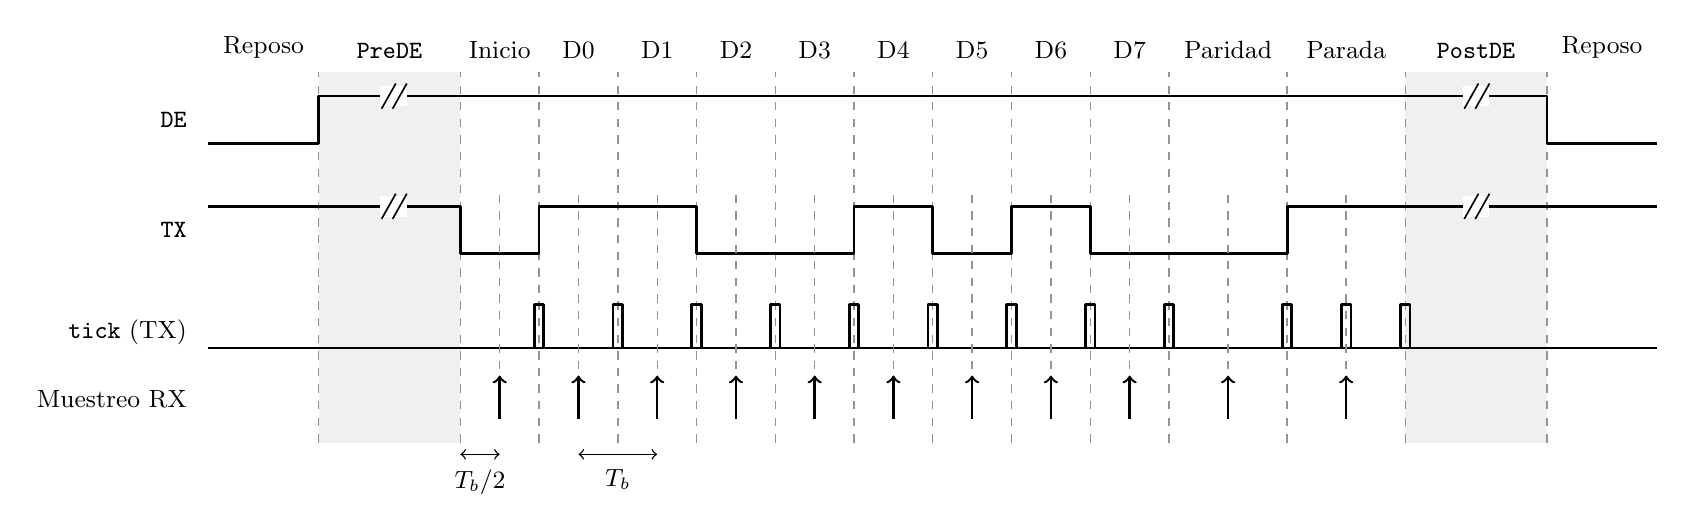
\begin{tikzpicture}[
        x=1cm, y=1cm,
        wave/.style={line width=1pt, line join=round},
        guide/.style={gray!85, dashed, line width=0.5pt},
        rowlbl/.style={font=\small, anchor=east},
        fieldlbl/.style={font=\small, anchor=south},
        meas/.style={<->, line width=0.5pt}]

    % --- Zonas no dibujadas a escala (PreDE / PostDE)
    \fill[gray!12] (1.4,0.20) rectangle (3.2,4.90);
    \fill[gray!12] (15.2,0.20) rectangle (17.0,4.90);

    % --- Líneas de separación de campo
    \foreach \x in {1.4,3.2,4.2,5.2,6.2,7.2,8.2,9.2,10.2,11.2,12.2,13.7,15.2,17.0}
        \draw[guide] (\x,0.20) -- (\x,4.90);

    % --- Etiquetas de campo
    \node[fieldlbl] at (0.7,4.95)   {Reposo};
    \node[fieldlbl] at (2.3,4.95)   {\texttt{PreDE}};
    \node[fieldlbl] at (3.7,4.95)   {Inicio};
    \foreach \i/\x in {0/4.7,1/5.7,2/6.7,3/7.7,4/8.7,5/9.7,6/10.7,7/11.7}
        \node[fieldlbl] at (\x,4.95) {D\i};
    \node[fieldlbl] at (12.95,4.95) {Paridad};
    \node[fieldlbl] at (14.45,4.95) {Parada};
    \node[fieldlbl] at (16.1,4.95)  {\texttt{PostDE}};
    \node[fieldlbl] at (17.7,4.95)  {Reposo};

    % --- DE
    \node[rowlbl] at (-0.15,4.30) {\texttt{DE}};
    \draw[wave] (0,4.0) -- (1.4,4.0) -- (1.4,4.6) -- (17.0,4.6) -- (17.0,4.0) -- (18.4,4.0);

    % --- TX (byte 0x53, LSB first: 1 1 0 0 1 0 1 0; paridad par = 0)
    \node[rowlbl] at (-0.15,2.90) {\texttt{TX}};
    \draw[wave] (0,3.2) -- (3.2,3.2) -- (3.2,2.6) -- (4.2,2.6)
                -- (4.2,3.2) -- (6.2,3.2) -- (6.2,2.6) -- (8.2,2.6)
                -- (8.2,3.2) -- (9.2,3.2) -- (9.2,2.6) -- (10.2,2.6)
                -- (10.2,3.2) -- (11.2,3.2) -- (11.2,2.6) -- (13.7,2.6)
                -- (13.7,3.2) -- (18.4,3.2);

    % --- Marcas de ruptura de escala
    \foreach \y in {4.6,3.2} {
        \fill[white] (2.18,\y-0.13) rectangle (2.52,\y+0.13);
        \draw[line width=0.6pt] (2.20,\y-0.16) -- (2.38,\y+0.16);
        \draw[line width=0.6pt] (2.34,\y-0.16) -- (2.52,\y+0.16);
        \fill[white] (15.93,\y-0.13) rectangle (16.27,\y+0.13);
        \draw[line width=0.6pt] (15.95,\y-0.16) -- (16.13,\y+0.16);
        \draw[line width=0.6pt] (16.09,\y-0.16) -- (16.27,\y+0.16);
    }

    % --- tick del NCO en el transmisor: un pulso por frontera de bit,
    %     y al doble de frecuencia durante el campo de parada
    \node[rowlbl] at (-0.15,1.60) {\texttt{tick} (TX)};
    \draw[wave] (0,1.4) -- (18.4,1.4);
    \foreach \x in {4.2,5.2,6.2,7.2,8.2,9.2,10.2,11.2,12.2,13.7,14.45,15.2}
        \draw[wave] (\x-0.06,1.4) -- (\x-0.06,1.95) -- (\x+0.06,1.95) -- (\x+0.06,1.4);

    % --- Instantes de muestreo del receptor: centro de cada bit
    \node[rowlbl] at (-0.15,0.75) {Muestreo RX};
    \foreach \x in {3.7,4.7,5.7,6.7,7.7,8.7,9.7,10.7,11.7,12.95,14.45} {
        \draw[guide] (\x,0.50) -- (\x,3.35);
        \draw[->, line width=0.9pt] (\x,0.50) -- (\x,1.05);
    }

    % --- Medidas de tiempo
    \draw[meas] (3.2,0.05) -- (3.7,0.05) node[midway, below=2pt, font=\small] {$T_b/2$};
    \draw[meas] (4.7,0.05) -- (5.7,0.05) node[midway, below=2pt, font=\small] {$T_b$};

    \end{tikzpicture}}%
    \shorthandon{<>}
    \caption{Cronograma de una trama completa en configuración 8E1, LSB \textit{first}.}
    \label{fig:cronograma_trama}
\end{figure}

\subsection{Normalización de la palabra recibida y almacenamiento} \label{sec:normalizacion_fifo}

Entre el receptor y el PS se sitúan dos bloques auxiliares. El registro de desplazamiento
convierte a paralelo los bits que entrega el receptor y \textbf{normaliza} la palabra: sea cual
sea la anchura y el orden de bits configurados, el primer bit de datos recibido acaba siempre en
\texttt{Q(0)} y la palabra queda alineada al LSB. Sus dos consumidores, la FIFO y el cálculo de
paridad esperada, pueden así ignorar la configuración del canal, y el software del PS recibe la
palabra en el mismo formato en los cinco anchos y en los dos órdenes posibles.

La FIFO es un bloque IP de 9~bits de dato y 512 de profundidad que almacena los mensajes ya
validados hasta que el PS los lee. Su habilitación de lectura se toma \textbf{a nivel} y no por
flanco, condición necesaria para el transporte por DMA descrito en la
sección~\ref{sec:transporte_desarrollo}: con la lectura a nivel la FIFO avanza exactamente en el
ciclo en que el consumidor acepta el dato.

La descripción RTL de ambos bloques, con los caminos de desplazamiento y la construcción de las
señales de escritura y lectura, se recoge en el apartado~\ref{anxC:rtl_fifo} del Anexo~\ref{anx:rtl}.

\subsection{Bloque de canal} \label{sec:bloque_canal}

\texttt{CONFIGURABLE\_SERIAL.vhd} instancia el transmisor, el receptor, el registro de
desplazamiento y la FIFO, y añade la lógica de acoplamiento entre ellos y con el PS:

\begin{itemize}
    \item \textbf{Registro de la línea de recepción.} La entrada \texttt{RD} se registra un ciclo
    antes de entrar al receptor, para no muestrear directamente una señal externa asíncrona
    respecto del reloj del sistema.

    \item \textbf{Detección de flanco de los mandos del PS.} \texttt{TX\_Send} y
    \texttt{Data\_read} llegan del PS como señales de nivel a través del AXI GPIO. Sendos
    detectores de flanco de dos etapas de registro los convierten en pulsos de un ciclo, que es lo
    que esperan los bloques internos.

    \item \textbf{Arranque de la transmisión.} El pulso de \texttt{Start} hacia el transmisor solo
    se emite si además el transmisor está libre (\texttt{EOT} activo), y en ese mismo ciclo la
    palabra presente en \texttt{Data\_in} se captura en un registro propio. De este modo el dato
    permanece estable durante toda la trama aunque el PS modifique el registro de escritura, y las
    peticiones que llegan con una transmisión en curso se ignoran en lugar de corromperla.

    \item \textbf{Adaptación del campo de parada.} El PS codifica los bits de parada en dos bits;
    transmisor y receptor los esperan como una cuenta de semiperíodos de tres bits. Una pequeña
    lógica combinacional traduce entre ambas representaciones.

    \item \textbf{Vector de depuración.} Una salida de cuatro bits agrupa las señales internas del
    camino de recepción (FIFO vacía, escritura en FIFO, bit válido y línea registrada), empleada
    únicamente para el diagnóstico en simulación.
\end{itemize}

Con el canal ya completo, la figura~\ref{fig:transceptor_bloques} recoge el conjunto: los bloques
descritos en los apartados anteriores, la lógica de acoplamiento que acaba de enumerarse y los
puertos con los que el canal se presenta al exterior, agrupados por función. Se aprecia en ella
que la palabra de configuración es común a los dos sentidos, que el camino de recepción encadena
receptor, registro de desplazamiento y FIFO antes de llegar al PS, y que \texttt{SLO} no entra en
la lógica: viaja del PS al pin del transceptor físico sin tocar el canal.

\begin{sidewaysfigure}
    \centering
    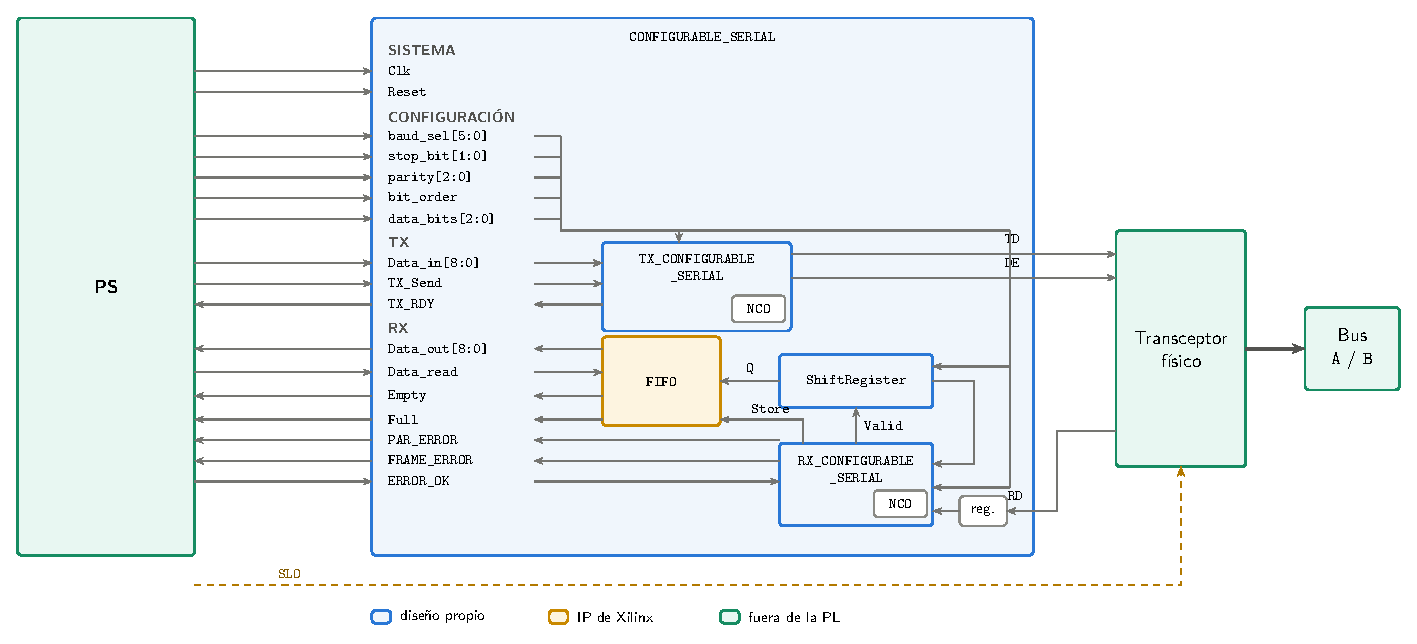
\includegraphics[width=0.97\textheight]{IMG/Desarrollo/diagrama_transceptor.pdf}
    \caption{Diagrama de bloques de un canal del transceptor serie configurable.}
    \label{fig:transceptor_bloques}
\end{sidewaysfigure}

\subsection{Bloque \textit{top} del transceptor}

\texttt{CONFIGURABLE\_SERIAL\_TOP.vhd} no añade funcionalidad: empaqueta el canal completo en dos
vectores, uno de entrada y otro de salida, para que pueda conectarse a los dos canales de un AXI
GPIO sin lógica adicional. El reparto de bits, que es el contrato entre la PL y el driver de RTEMS
descrito en la sección siguiente, se recoge en la tabla~\ref{tab:mapa_bits_top}.

\begin{table}[H]
    \centering
    \begin{tabular}{llp{0.46\textwidth}}
        \hline
        \textbf{Bits} & \textbf{Campo} & \textbf{Función} \\
        \hline
        \multicolumn{3}{l}{\textit{Vector de configuración y escritura (PS $\rightarrow$ PL), 28 bits}} \\
        \hline
        8:0   & \texttt{Data\_in}   & Palabra a transmitir. \\
        9     & \texttt{TX\_Send}   & Petición de transmisión. \\
        10    & \texttt{ERROR\_OK}  & Reconocimiento de las banderas de error. \\
        11    & \texttt{Data\_read} & Lectura de la FIFO de recepción. \\
        17:12 & \texttt{baud\_sel}  & Índice de velocidad. \\
        19:18 & \texttt{stop\_bit}  & Bits de parada. \\
        22:20 & \texttt{parity}     & Modo de paridad. \\
        25:23 & \texttt{data\_bits} & Número de bits de datos. \\
        26    & \texttt{bit\_order} & Orden de bits. \\
        27    & \texttt{SLO}        & Control del limitador de \textit{slew rate} del transceptor
                                      físico. \\
        \hline
        \multicolumn{3}{l}{\textit{Vector de estado y lectura (PL $\rightarrow$ PS), 14 bits}} \\
        \hline
        8:0   & \texttt{Data\_out}    & Palabra recibida. \\
        9     & \texttt{Empty}        & FIFO de recepción vacía. \\
        10    & \texttt{Full}         & FIFO de recepción llena. \\
        11    & \texttt{PAR\_ERROR}   & Error de paridad. \\
        12    & \texttt{FRAME\_ERROR} & Error de trama. \\
        13    & \texttt{TX\_RDY}      & Transmisor libre. \\
        \hline
    \end{tabular}
    \caption[Reparto de bits de los vectores de interfaz]{Reparto de bits de los vectores de
    interfaz del bloque \texttt{CONFIGURABLE\_SERIAL\_TOP}.}
    \label{tab:mapa_bits_top}
\end{table}

Junto a esos dos vectores, el bloque expone las líneas físicas del canal (\texttt{TD},
\texttt{RD}, \texttt{DE} y \texttt{SLO}) y una salida auxiliar de dos bits que duplica
\texttt{TX\_RDY} y \texttt{Empty}. Esta última es la que se lleva al controlador de interrupciones,
para que el PS pueda ser avisado tanto de la llegada de datos como de la disponibilidad del
transmisor sin tener que sondear el vector de estado. La salida \texttt{SLO} es una conexión
directa desde el bit~27 del vector de configuración hasta el pin del transceptor físico: no
interviene en la lógica del transceptor en VHDL.

\subsubsection{Envoltorios de nivel superior}

El canal así empaquetado es la unidad que reutilizan los tres envoltorios de nivel superior
presentes en el repositorio, cada uno asociado a una de las arquitecturas de transporte entre el
PS y la PL:

\begin{itemize}
    \item \texttt{MULTI\_SERIAL\_CORE.vhd} agrupa hasta catorce instancias del bloque \textit{top}
    en un único IP, con las interfaces de todos los canales aplanadas en vectores de ancho fijo y
    un par de genéricos por canal que ocultan los pines \texttt{DE} y \texttt{SLO} que no se
    cablean; es el bloque de catorce canales de la arquitectura basada en AXI GPIO.

    \item \texttt{SERIAL\_CHANNEL\_IP.vhd} envuelve un solo canal como IP independiente, con esos
    mismos genéricos, para que los canales puedan instanciarse y conectarse uno a uno en el
    \textit{Block Design} en lugar de como un bloque monolítico.

    \item \texttt{UART\_AXIS\_TOP.vhd} sustituye la interfaz paralela por un registro de
    configuración AXI-Lite y dos canales AXI-Stream (uno de transmisión y otro de recepción, este
    último con \textit{TDEST} fijado al índice de canal y \textit{TLAST} por byte), que es lo que
    permite conectar el transceptor directamente a un controlador de DMA.
\end{itemize}

Ninguno de los tres modifica el comportamiento del transceptor descrito en esta sección: cambian
únicamente la forma en que sus dos vectores se presentan al PS. Su papel dentro de cada
arquitectura se detalla en la sección~\ref{sec:transporte_desarrollo}.

\subsection{Verificación en simulación del canal completo}
\label{sec:verificacion_canal}

Cada bloque descrito en los apartados anteriores tiene su propio \textit{testbench}. La
comprobación que realmente acredita el transceptor es la del canal completo. Es la única que
ejercita a la vez las dos máquinas de estados, la normalización del registro de desplazamiento y la
coherencia entre la paridad generada y la esperada. El \textit{testbench}
\texttt{tb\_CONFIGURABLE\_SERIAL\_TOP.vhd}, en \texttt{tfm/01\_ip\_serie/testbench/} del
repositorio del proyecto~\cite{repo_tfm}, conecta la salida \texttt{TX} del canal a su propia
entrada \texttt{RD}. \textbf{Recorre el espacio de configuración completo} a 921\,600~baudios:
cinco anchuras de palabra (5 a 9 bits) $\times$ dos órdenes de bit $\times$ tres campos de parada
(1, 1,5 y 2) $\times$ cinco modos de paridad, es decir \textbf{150 configuraciones}, con tres
tramas de contenido distinto en cada una. En total, \textbf{450 tramas} comparadas dato a dato
entre lo enviado y lo recibido:

\begin{lstlisting}[style=terminal, caption={Salida de la simulación de \texttt{tb\_CONFIGURABLE\_SERIAL\_TOP.vhd} (extracto)}]
==== TB START: TX->RX loopback tests ====
==== sending byte ====
PASS cfg bits=5 order='0' stop=1 par=0 sent=11 rec=11
==== sending byte ====
PASS cfg bits=5 order='0' stop=1 par=0 sent=12 rec=12
==== sending byte ====
PASS cfg bits=5 order='0' stop=1 par=0 sent=13 rec=13
==== sending byte ====
PASS cfg bits=5 order='0' stop=1 par=1 sent=28 rec=28
...
PASS cfg bits=8 order='1' stop=2 par=4 sent=118 rec=118
...
==== sending byte ====
PASS cfg bits=9 order='1' stop=3 par=4 sent=132 rec=132
==== sending byte ====
PASS cfg bits=9 order='1' stop=3 par=4 sent=133 rec=133
==== sending byte ====
PASS cfg bits=9 order='1' stop=3 par=4 sent=134 rec=134
==== TESTS FINISHED ====
Passed = 450 / Total = 450
\end{lstlisting}

Las 450 tramas se recuperaron íntegras. Ninguna disparó las banderas \texttt{PAR\_ERROR} ni
\texttt{FRAME\_ERROR}, que el \textit{testbench} vigilaba trama a trama. El dato relevante no es
tanto el número como su cobertura. Al completar el barrido quedó comprobado que el transmisor y
el receptor coinciden en todos sus bloques: el multiplexor de serialización, el decodificador de
anchura, la red de paridad y los dos caminos de desplazamiento del registro. Esta coincidencia se
cumple \textbf{en todas} las combinaciones que el PS puede programar, y no solo en la
configuración 8N1 habitual.

Por legibilidad, en esta transcripción y en las que siguen se reproducen únicamente las líneas de
\texttt{report} del \textit{testbench}. Se omiten las marcas de tiempo, iteración e instancia que
el simulador antepone a cada una.

\subsection{Bloque Zynq UltraScale+ MPSoC}

Para que el proyecto en Vivado funcione correctamente, es importante aplicar el \textit{preset} al
bloque IP Zynq UltraScale+ antes de añadir el resto de elementos. El \textit{preset} aplica
configuraciones de relojes y alimentación cruciales para el correcto funcionamiento de la PL.

% ---------------------------------------------------------------------------
\section{Herramientas de apoyo al desarrollo del transceptor}
% ---------------------------------------------------------------------------

\subsection{Generación de transceptores con TCL}

Se desarrolló un script de TCL, \texttt{new\_generate\_transceivers.tcl}, que permite generar y
conectar automáticamente un número deseado de transceptores en el \textit{Block Design} de Vivado.
Recibe el número de instancias y los nombres del bloque Zynq y del \textit{SmartConnect} a los que
engancharse, y a partir de ahí añade y conecta el resto de los bloques necesarios: un AXI GPIO de
doble canal por transceptor, el controlador de interrupciones común, un bloque de solo lectura con
los metadatos del sistema que consulta el driver, y la asignación de direcciones en el mapa de
memoria del PS. Parte de un proyecto que ya tenga las fuentes .vhd del transceptor, el
\textit{Block Design} creado y el bloque IP Zynq UltraScale+ MPSoC configurado. El script está en
\texttt{tfm/01\_ip\_serie/scripts/} dentro del repositorio del proyecto~\cite{repo_tfm}, y cada
proyecto de Vivado conserva su copia en el subdirectorio \texttt{scripts/} correspondiente.

\subsection{Generación de proyecto con TCL}

También se desarrolló otro script de TCL, \texttt{new\_rebuild\_all.tcl}, que regenera el proyecto
entero de Vivado con un número determinado de transceptores, partiendo desde cero. Crea el
proyecto para la ZCU102, añade las fuentes y las restricciones, instancia y configura el bloque
Zynq, invoca al generador de transceptores anterior, valida el diseño y genera el \textit{wrapper}.
El proyecto queda así listo para lanzar la síntesis y la generación del \textit{bitstream}. Esto
permite reproducir exactamente cualquier configuración sin necesidad de guardar el proyecto
de Vivado completo en el repositorio.

% ---------------------------------------------------------------------------
\section{Diseño del driver serie en RTEMS (PS)} \label{sec:driver_rtems}
% ---------------------------------------------------------------------------

Completado el transceptor en la PL, se continuó con su contraparte en el PS: los ficheros
\texttt{transceiver.c} y \texttt{transceiver.h}. Es un driver para RTEMS que habla con el hardware a
través del AXI GPIO de cada canal y expone a la aplicación una API pública sencilla, la misma para
los catorce canales. Las subsecciones siguientes lo describen de fuera hacia dentro. Primero se
presenta la API que ve la aplicación. Después, el mapa de registros con el que el driver dialoga
con la PL. Por último, se explica cómo gestiona por dentro la transmisión y la recepción sin
bloquear al procesador.

Este driver se planteó como prueba de concepto: el objetivo era que funcionase, sin requisitos
impuestos y sin optimizar nada. Funcionó, y con eso queda cumplido su propósito.

\subsection{API pública}

Para la aplicación, cada canal serie es un objeto \texttt{Transceiver} sobre el que actúan las seis
funciones de su API pública. El driver oculta el reparto de memoria, la gestión de interrupciones y
la sincronización entre tareas: el código de usuario se limita a abrir el canal, fijar su
configuración de protocolo y recibir o transferir bytes. Las funciones, con su tipo de retorno, son:

\begin{itemize}
    \item \texttt{uint32\_t Transceiver\_Global\_INIT(void)}
    \item \texttt{rtems\_status\_code Transceiver\_Init(dev, id, cfg)}
    \item \texttt{void Transceiver\_SetRxCallback(dev, cb, arg)}
    \item \texttt{size\_t Transceiver\_Read(dev, buf, maxlen)}
    \item \texttt{int Transceiver\_Send(dev, data, len)}
    \item \texttt{int Transceiver\_SendString(dev, s)}
\end{itemize}

\texttt{Transceiver\_Global\_INIT()} se invoca una sola vez al arranque. Descubre cuántos canales
trae el \textit{bitstream}, prepara el controlador de interrupciones, instala la rutina de
interrupción común y devuelve el número de canales encontrados.

\texttt{Transceiver\_Init()} se llama una vez por canal. Recibe una estructura
\texttt{Transceiver\_\allowbreak Config\_t} con la tasa de baudios, los bits de datos, la paridad, los bits de
parada y el orden de bits, y deja el canal listo para operar.

\texttt{Transceiver\_SetRxCallback()} registra la función de recepción, el \textit{callback}. La
escribe el usuario y su contenido es libre. El driver la invoca cada vez que hay bytes nuevos
disponibles. Es la aplicación la que decide qué hacer con ellos: leerlos en el acto, despertar a
otra tarea, contabilizar la recepción o cualquier otra cosa. Es solo una notificación: cuando se
dispara, el driver ya ha sacado del hardware los bytes y los tiene disponibles.

\texttt{Transceiver\_Read()} extrae del \textit{buffer} de recepción hasta \texttt{maxlen} bytes ya
recibidos, devuelve cuántos ha copiado y no bloquea aunque no haya ninguno. Es la función con la que
la aplicación retira los datos, normalmente desde el \textit{callback} o desde una tarea propia.

\texttt{Transceiver\_Send()} encola los bytes a transmitir y retorna de inmediato, sin esperar a que
salgan por la línea. Devuelve cuántos aceptó, o un error si el \textit{buffer} de salida estaba
lleno. \texttt{Transceiver\_SendString()} es la misma operación para cadenas terminadas en nulo.

\subsection{Interfaz con el hardware}

El driver y la PL se comunican a través de un único bloque AXI GPIO por canal, configurado como
doble canal y mapeado en 4~KB del espacio de direcciones del procesador. Los dos canales tienen
sentido fijo. El canal~1, de 28 bits, escribe del PS a la PL. El canal~2, de 14 bits, lee de la PL
al PS. Cada uno se maneja con su registro de datos, situado en los desplazamientos \texttt{0x00} y
\texttt{0x08} respecto de la dirección base de la instancia. Toda la interacción con el hardware
se reduce así a escribir y leer dos palabras de 32 bits.

El registro de escritura reúne el dato a transmitir, tres bits de control y los campos de
configuración de protocolo. El de lectura reúne el byte recibido y las banderas de estado. La
tabla~\ref{tab:mapa_registros_gpio} recoge el reparto de bits.

\begin{table}[H]
    \centering
    \small
    \begin{tabular}{@{}c l c l@{}}
        \hline
        \multicolumn{2}{c}{\textbf{Escritura (PS $\rightarrow$ PL)}} &
        \multicolumn{2}{c}{\textbf{Lectura (PL $\rightarrow$ PS)}} \\
        \textbf{Bits} & \textbf{Campo} & \textbf{Bits} & \textbf{Campo} \\
        \hline
        8:0   & Dato a transmitir   & 8:0 & Byte recibido \\
        9     & \texttt{SEND}       & 9   & \texttt{RX\_EMPTY} \\
        10    & \texttt{ERROR\_OK}  & 10  & \texttt{RX\_FULL} \\
        11    & \texttt{DATA\_READ} & 11  & \texttt{PARITY\_ERROR} \\
        17:12 & Tasa de baudios     & 12  & \texttt{FRAME\_ERROR} \\
        19:18 & Bits de parada      & 13  & \texttt{TX\_RDY} \\
        22:20 & Paridad             &     & \\
        25:23 & Bits de datos       &     & \\
        26    & Orden de bits       &     & \\
        27    & \texttt{SLO}        &     & \\
        \hline
    \end{tabular}
    \caption{Mapa de bits de los dos canales del AXI GPIO de una instancia.}
    \label{tab:mapa_registros_gpio}
\end{table}

Los campos de configuración de protocolo se escriben una sola vez, en
\texttt{Transceiver\_\allowbreak Init()}, y permanecen fijos mientras el canal está abierto. El driver guarda
esa palabra y la reutiliza como base cada vez que toca los bits inferiores, para no alterar la
configuración al transmitir. Los bits de control funcionan como pulsos, no como niveles. Para
transmitir se deposita el byte en los bits 8:0 y se lleva \texttt{SEND} a uno y de vuelta a cero, lo
que ordena al transmisor cargar el dato. Para consumir un byte recibido se lee el canal de entrada y
se pulsa \texttt{DATA\_READ}, que hace avanzar la FIFO de recepción. \texttt{ERROR\_OK} es el
reconocimiento equivalente para las banderas de error. En sentido contrario, \texttt{RX\_EMPTY}
indica si queda algo por leer y \texttt{TX\_RDY} que el transmisor ha terminado el byte en curso y
admite el siguiente.

\textbf{Descubrimiento del mapa de direcciones.} Ninguna dirección de canal está escrita en el
código. En la dirección fija \texttt{0xA0020000} se sitúa un AXI GPIO adicional, de solo lectura.
Sus dos entradas están cableadas en la PL a constantes que el script de generación calcula al
construir el \textit{bitstream}. Ese bloque de información publica tres valores:

\begin{itemize}
    \item \textbf{Número de transceptores} instanciados, $N$, en los bits 15:0 del canal~1.
    \item \textbf{\textit{Stride}}, en los bits 31:16 del canal~1: la distancia en bytes entre la
          dirección base de una instancia y la de la siguiente, 4~KB en este diseño.
    \item \textbf{Dirección base} del primer transceptor, en el canal~2.
\end{itemize}

Las instancias se asignan de forma contigua a partir de esa base, y el AXI INTC compartido por todas
ellas queda inmediatamente después de la última. Con los tres valores, leídos al arrancar en
\texttt{Transceiver\_Global\_INIT()}, el driver deduce el resto del mapa con dos cuentas:

\[
    \text{base}_i = \text{base} + i \cdot \text{\textit{stride}}, \quad i = 0,\dots,N-1
    \qquad
    \text{base}_{\text{INTC}} = \text{base} + N \cdot \text{\textit{stride}}
\]

De este modo el mismo binario RTEMS funciona sobre cualquier \textit{bitstream}, desde un único
canal hasta los catorce, sin recompilar. Basta con que el hardware declare cuántas instancias trae
y dónde empiezan.

\textbf{Bit \texttt{SLO}.} El bit \texttt{SLO} del registro de escritura no actúa sobre la lógica en
VHDL: se propaga hasta el pin \texttt{SLO} del chip transceptor de la PCB. El driver se limita a
exponerlo. Su efecto eléctrico y la cuantificación de su impacto sobre la velocidad máxima del
enlace se tratan en la caracterización de la placa (sección~\ref{sec:pcb_slo}).

\subsection{Gestión interna de la transmisión}

La figura~\ref{fig:driver_camino_datos} resume el recorrido interno de un byte en cada sentido.
Esta subsección se ocupa de la transmisión, y la siguiente, de la recepción.

\begin{figure}[htbp]
    \centering
    % babel-spanish activa < y >, que TikZ necesita para las puntas de flecha
    \shorthandoff{<>}%
    \resizebox{\textwidth}{!}{%
    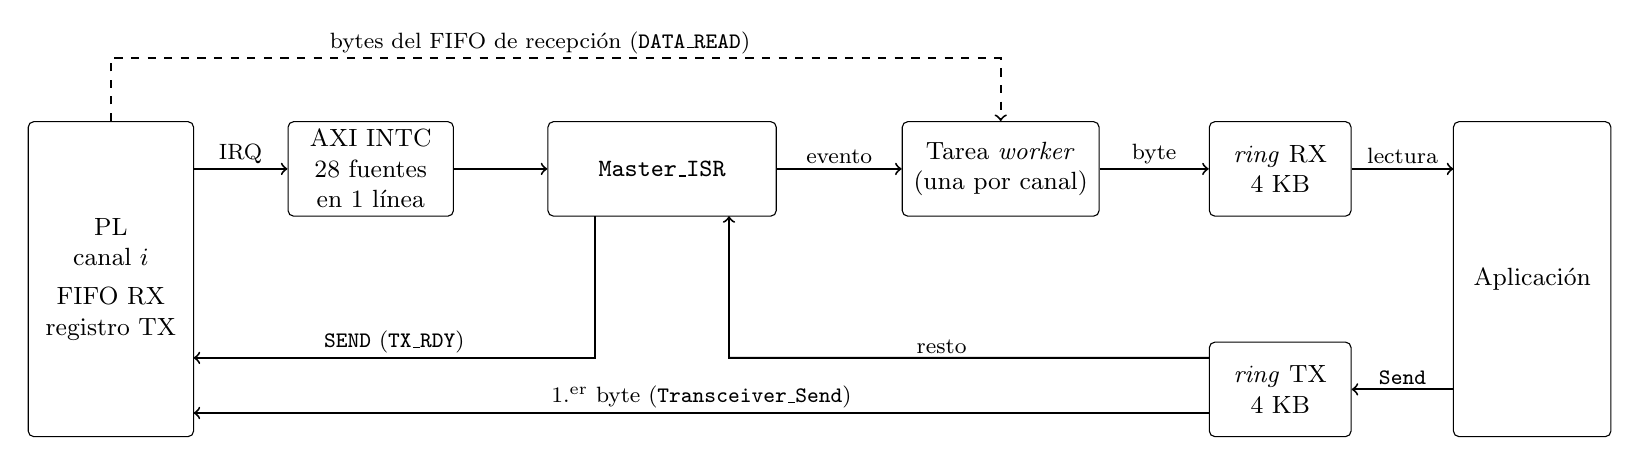
\begin{tikzpicture}[
        x=1cm, y=1cm,
        box/.style={draw, rounded corners=2pt, align=center, font=\small,
                    inner sep=3pt, minimum height=1.2cm},
        tall/.style={box, minimum height=4.0cm},
        flow/.style={->, line width=0.7pt},
        back/.style={->, line width=0.7pt, dashed},
        lbl/.style={font=\footnotesize, inner sep=1.5pt}]

    \node[tall, minimum width=2.1cm] (pl)   at (1.05,2.0)  {PL\\canal $i$\\[3pt]FIFO RX\\registro TX};
    \node[box,  minimum width=2.1cm] (intc) at (4.35,3.4)  {AXI INTC\\28 fuentes\\en 1 línea};
    \node[box,  minimum width=2.9cm] (isr)  at (8.05,3.4)  {\texttt{Master\_ISR}};
    \node[box,  minimum width=2.5cm] (wkr)  at (12.35,3.4) {Tarea \textit{worker}\\(una por canal)};
    \node[box,  minimum width=1.8cm] (rxr)  at (15.90,3.4) {\textit{ring} RX\\4~KB};
    \node[box,  minimum width=1.8cm] (txr)  at (15.90,0.6) {\textit{ring} TX\\4~KB};
    \node[tall, minimum width=2.0cm] (app)  at (19.10,2.0) {Aplicación};

    % --- Recepción
    \draw[flow] (2.1,3.4)     -- (intc.west) node[lbl, above, midway] {IRQ};
    \draw[flow] (intc.east)   -- (isr.west);
    \draw[flow] (isr.east)    -- (wkr.west)  node[lbl, above, midway] {evento};
    \draw[flow] (wkr.east)    -- (rxr.west)  node[lbl, above, midway] {byte};
    \draw[flow] (rxr.east)    -- (18.1,3.4)  node[lbl, above, midway] {lectura};
    \draw[back] (pl.north) -- ++(0,0.8) -| (wkr.north);
    \node[lbl, above] at (6.5,4.8) {bytes del FIFO de recepción (\texttt{DATA\_READ})};

    % --- Transmisión
    \draw[flow] (18.1,0.6) -- (txr.east) node[lbl, above, midway] {\texttt{Send}};
    % primer byte: escrito directamente por Transceiver_Send, sin pasar por la ISR
    \draw[flow] ([yshift=-0.3cm]txr.west) -- (2.1,0.3);
    \node[lbl, above] at (8.55,0.3) {1.\textsuperscript{er} byte (\texttt{Transceiver\_Send})};
    % resto de la cola: la va drenando la Master_ISR al recibir TX_RDY
    \draw[flow] ([yshift=0.4cm]txr.west) -- (8.90,1.0) -- (8.90,2.8);
    \node[lbl, above] at (11.6,1.0) {resto};
    \draw[flow] (7.20,2.8) -- (7.20,1.0) -- (2.1,1.0);
    \node[lbl, above] at (4.65,1.0) {\texttt{SEND} (\texttt{TX\_RDY})};

    \end{tikzpicture}}%
    \shorthandon{<>}
    \caption{Camino de un byte entre la lógica programable y la aplicación.}
    \label{fig:driver_camino_datos}
\end{figure}

Cada canal dispone de un \textit{buffer} circular de salida de 4~KB, tamaño que da margen para
ráfagas a las tasas más altas soportadas, hasta 4~Mbaudios. \texttt{Transceiver\_Send()} copia ahí
los bytes de la aplicación. Si el transmisor estaba en reposo, escribe el primero directamente en
el registro de escritura para poner en marcha el hardware. La tarea que llama no se bloquea.

El resto de la ráfaga lo va sacando la rutina de interrupción. Los catorce canales comparten un
único controlador AXI INTC, que concentra sus veintiocho fuentes de interrupción (la de recepción y
la de transmisión de cada canal) en una sola línea hacia el PS. Una única rutina,
\texttt{Master\_ISR}, atiende esa línea. Cuando el transmisor de un canal termina de emitir un
byte, activa su señal \texttt{TX\_RDY}. La \texttt{Master\_ISR} lee el registro de interrupciones
pendientes y localiza el canal en la tabla de instancias \texttt{g\_instances[]} mediante un
índice directo, sin listas enlazadas ni búsquedas en contexto de interrupción. Toma entonces el
siguiente byte de su cola y lo escribe. Cuando la cola queda vacía, marca el canal como libre.

En transmisión, por tanto, la rutina de interrupción sí mueve el dato, pero es la escritura de un
único byte por interrupción. Su coste está acotado y no compromete la latencia del sistema. Un
semáforo binario serializa las llamadas concurrentes de varias tareas a \texttt{Transceiver\_Send()}
sobre el mismo canal. El acceso al \textit{buffer} frente a la \texttt{Master\_ISR} se protege
inhibiendo un instante las interrupciones durante el encolado.

\subsection{Gestión interna de la recepción}

La recepción sigue el patrón de procesado diferido recomendado en RTEMS: la rutina de interrupción
hace lo imprescindible y delega el grueso del trabajo en una tarea ordinaria. Esa tarea, la
\textit{worker}, es una tarea de RTEMS: un hilo con su propia pila y prioridad que el planificador
del sistema operativo de tiempo real gestiona junto con las demás. Se ejecuta cuando le
corresponde, cede la CPU mientras espera y no carga al núcleo más que con un cambio de contexto.
Hay una \texttt{Rx\_Worker\_Task} por canal, creada en \texttt{Transceiver\_Init()} y bloqueada a la
espera de trabajo.

Cuando llega un byte por la línea, el receptor del canal genera una interrupción. La
\texttt{Master\_ISR} la reconoce, inhibe temporalmente esa fuente en el INTC y envía un evento
RTEMS a la \texttt{Rx\_Worker\_Task} del canal. Ahí acaba el trabajo en contexto de interrupción. La
tarea despierta y vacía el FIFO del hardware byte a byte hacia el \textit{buffer} circular de
recepción, también de 4~KB, confirmando cada extracción con el bit \texttt{DATA\_READ}. Al agotar el
FIFO invoca el \textit{callback} que la aplicación haya registrado, vuelve a habilitar la
interrupción y se bloquea de nuevo. La aplicación recoge los bytes cuando puede con
\texttt{Transceiver\_Read()}. Un semáforo binario por canal protege el \textit{buffer} de recepción
frente al acceso simultáneo de la \textit{worker} y la aplicación.

Esa copia, de duración variable, corre ya como tarea sujeta al planificador y no en la rutina de
interrupción. Por ello, la latencia de interrupción del sistema no depende del volumen de datos
que llegue por las líneas serie.
